Die Geschwindigkeit ist die Steigung des $s(t)$-Graphen. Man prüft die Skizze Stück für Stück:
\begin{center}
\begin{tabular}{c|c|c|c}
Stück & $\Delta s$ & $\Delta t$ & $v = \Delta s/\Delta t$ \\
\hline
1 & \SI{6}{\meter} & \SI{2}{\second} & \SI{3}{\meter\per\second} \\
2 & \SI{0}{\meter} & \SI{2}{\second} & \SI{0}{\meter\per\second} \\
3 & \SI{-4}{\meter} & \SI{1}{\second} & \SI{-4}{\meter\per\second} \\
4 & \SI{0}{\meter} & \SI{2}{\second} & \SI{0}{\meter\per\second} \\
5 & \SI{3}{\meter} & \SI{2}{\second} & \SI{1.5}{\meter\per\second}
\end{tabular}
\end{center}
\begin{abcliste}
\abc $\result{\text{Stück 4}}$ (von \tFourO\ bis \tFiveO) ist falsch, alle anderen stimmen.

\abc Im Stück 4 ist der $s(t)$-Graph waagrecht bei $s = \sRestO$: Der Körper ruht. Die Schülerin hat die $\result{\text{Höhe des } s(t)\text{-Graphen statt seiner Steigung}}$ übernommen und \SI{2}{\meter\per\second} gezeichnet. Richtig ist $v = 0$: Ein Körper, der still steht, hat keine Geschwindigkeit, egal wo er steht. Die richtige Skizze:
\begin{center}
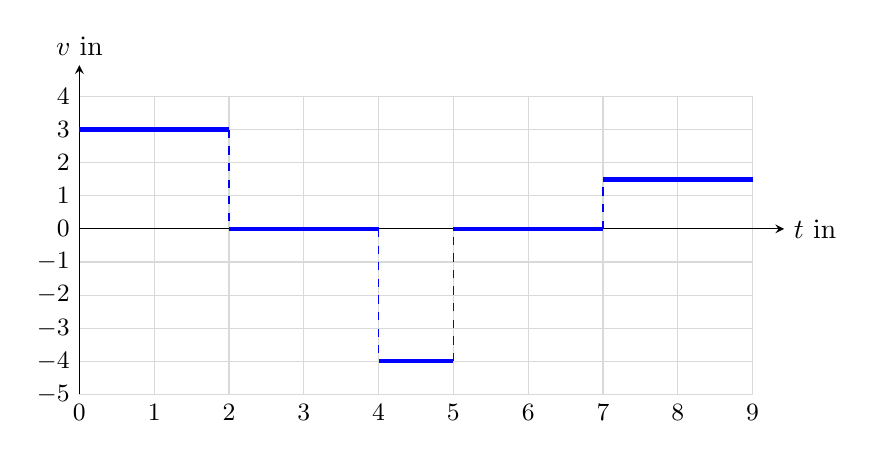
\begin{tikzpicture}[>=stealth, x=0.95cm, y=0.42cm]
 \draw[gray!30] (0,-5) grid[xstep=1, ystep=1] (9,4);
 \draw[->] (0,0) -- (9.421,0) node[right] {$t$ in \si{\second}};
 \draw[->] (0,-5) -- (0,4.952) node[above] {$v$ in \si{\meter\per\second}};
 \foreach \tk in {0,1,2,3,4,5,6,7,8,9} \node[below] at (\tk,-5) {\small $\tk$};
 \foreach \yk in {-5,-4,-3,-2,-1,0,1,2,3,4} \node[left] at (0,\yk) {\small $\yk$};

 \draw[ultra thick, blue] (0,3) -- (2,3);
 \draw[ultra thick, blue] (2,0) -- (4,0);
 \draw[ultra thick, blue] (4,-4) -- (5,-4);
 \draw[ultra thick, blue] (5,0) -- (7,0);
 \draw[ultra thick, blue] (7,1.5) -- (9,1.5);
 \draw[blue, dashed] (2,3) -- (2,0) (4,0) -- (4,-4) (5,-4) -- (5,0) (7,0) -- (7,1.5);
\end{tikzpicture}
\end{center}
\end{abcliste}
